\documentclass{standalone}
\usepackage{tikz}
\usetikzlibrary{positioning,arrows.meta,shapes,decorations.pathreplacing}
\usepackage{amssymb}

\begin{document}
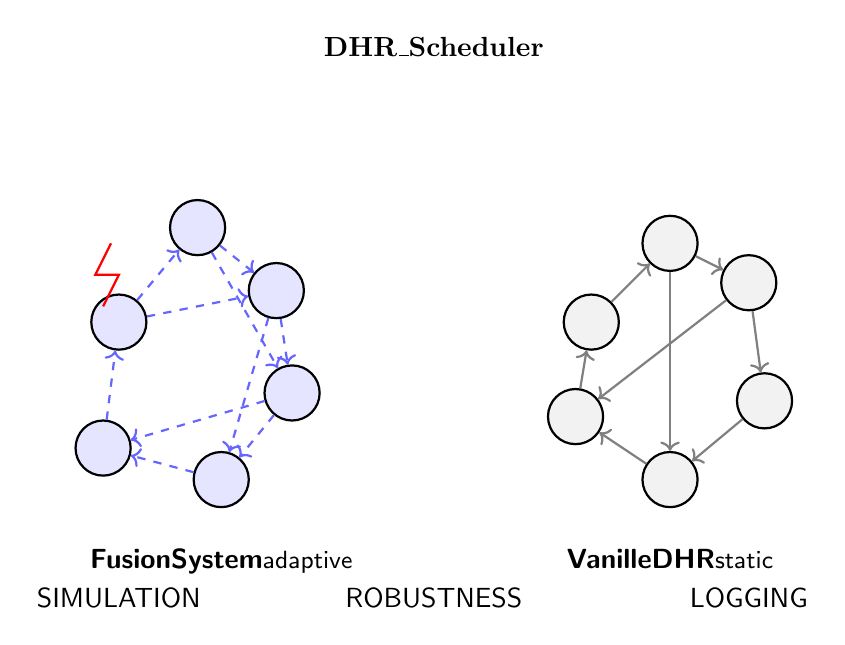
\begin{tikzpicture}[
        node/.style={circle, draw, thick, minimum size=7mm},
        dashedline/.style={->, thick, dashed},
        solidline/.style={->, thick},
        attack/.style={thick, red},
        font=\sffamily
    ]

    % FusionSystem (left)
    \node[node, fill=blue!10] (a1) at (-4,2) {};
    \node[node, fill=blue!10] (a2) at (-3,3.2) {};
    \node[node, fill=blue!10] (a3) at (-2,2.4) {};
    \node[node, fill=blue!10] (a4) at (-1.8,1.1) {};
    \node[node, fill=blue!10] (a5) at (-2.7,0) {};
    \node[node, fill=blue!10] (a6) at (-4.2,0.4) {};

    % FusionSystem connections
    \foreach \i/\j in {a1/a2,a1/a3,a2/a3,a2/a4,a3/a4,a3/a5,a4/a5,a5/a6,a6/a1,a4/a6} {
            \draw[dashedline, blue!60] (\i) -- (\j);
        }

    % Attack symbol
    \draw[attack] (-4.2,2.2) -- (-4.0,2.6) -- (-4.3,2.6) -- (-4.1,3.0);

    % FusionSystem label
    \node[below=0.4cm of a5] (fslabel) {\textbf{FusionSystem}\\\small adaptive};

    % VanilleDHR (right)
    \node[node, fill=gray!10] (b1) at (2,2) {};
    \node[node, fill=gray!10] (b2) at (3,3) {};
    \node[node, fill=gray!10] (b3) at (4,2.5) {};
    \node[node, fill=gray!10] (b4) at (4.2,1) {};
    \node[node, fill=gray!10] (b5) at (3,0) {};
    \node[node, fill=gray!10] (b6) at (1.8,0.8) {};

    % VanilleDHR connections
    \foreach \i/\j in {b1/b2,b2/b3,b3/b4,b4/b5,b5/b6,b6/b1,b2/b5,b3/b6} {
            \draw[solidline, gray] (\i) -- (\j);
        }

    % VanilleDHR label
    \node[below=0.4cm of b5] (vhlabel) {\textbf{VanilleDHR}\\\small static};

    % Global title
    \node[font=\bfseries, yshift=1.5cm] at (0,4) {DHR\_Scheduler};

    % Bottom labels
    \node at (-4,-1.5) {SIMULATION};
    \node at (0,-1.5) {ROBUSTNESS};
    \node at (4,-1.5) {LOGGING};

\end{tikzpicture}
\end{document}
